\subsection{Comparison of methods}

As discussed above, computing worst-case running time bounds is difficult for both expansion methods. Thus, we empirically examine the running time of the methods presented. 

We first introduce the dataset we will use to compare the methods outlined above: the noisy unit circle (NUC) with fluctuation $\alpha$. Points are taken uniformly at random from the annulus with outer radius $1 + \alpha/2$ and inner radius $1 - \alpha/2$ (we will take $\alpha = 0.1$ unless otherwise stated). The underlying population of this test set is homeomorphic to the open cylinder $S^1 \times (0,1)$.

Three experiments were conducted on an instance of NUC to investigate the performance of the methods outlined above for \textsc{$\hat\varepsilon$-VRFilt}:
\begin{enumerate}
    \item investigating the running time of the brute force skeleton method and the method provided by sklearn \cite{scikit-learn} with varying point count;
    \item investigating the running time of the three expansion methods with varying $\hat\varepsilon$; and
    \item investigating the running time of the two (non-brute force) expansion methods with varying $\hat\varepsilon$.
\end{enumerate}

For experiment (i), we take $\hat\varepsilon = 0.01$. Note that the method provided by sklearn does not use the state-of-the-art hierarchical navigable small-world networks. In fact, it does not use a single method. The package will scan the underlying dataset and pick the optimal algorithm, one possible algorithm uses BBD-trees as mentioned from \textcite{arya1998optimal}. For experiments (ii) and (iii) our test set consists of 1000 points and we calculate expansion up to 10 dimensions. 

\begin{figure}
    \makebox[\textwidth][c]{
        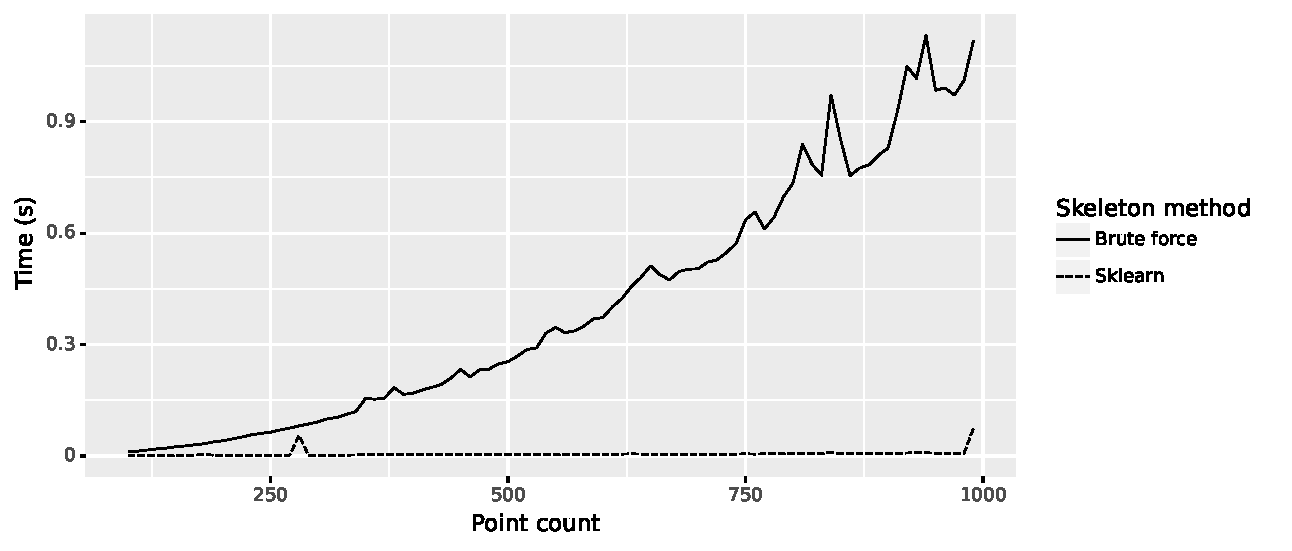
\includegraphics[width=1.2\textwidth]{content/4-comp-top/images/1-skeleton-methods}
    }
    \caption{A plot of the performance of two skeleton methods (with varying point count): the brute force method and the method provided by sklearn. The test set is the noisy unit circle (with radius fluctuation 0.1) with $\varepsilon = 0.01$.}
    \label{fig:skeleton-methods}
\end{figure}

Figure \ref{fig:skeleton-methods} shows the results of experiment (i), and we can clearly see that the brute force methods has poor performance. This figure does not show the performance of the sklearn method at higher point counts: the sklearn method (typically) runs in under a second for test sets of size \num{1000000} and higher (depending on $\hat\varepsilon$). From this, it is reasonable to conclude that the expansion method is the bottleneck in calculating the Vietoris-Rips filtration (the subsequent experiments reaffirm this claim).

\begin{figure}
    \makebox[\textwidth][c]{
        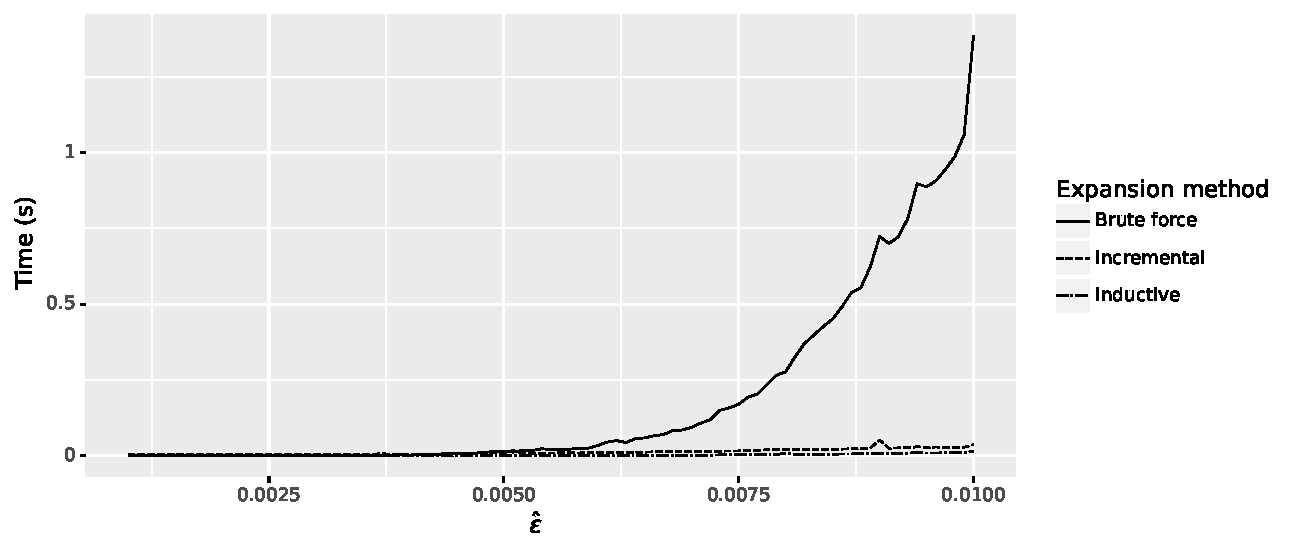
\includegraphics[width=1.2\textwidth]{content/4-comp-top/images/1-initial-expansion-methods}
    }
    \caption{A plot of the performance of three expansion methods (with varying $\varepsilon$): the brute force method, the inductive algorithm, and the incremental algorithm. The test set is is the noisy unit circle (with radius fluctuation 0.1) and the expansion is calculated up to 10 dimensions.}
    \label{fig:initial-expansion-methods}
\end{figure}

Figure \ref{fig:initial-expansion-methods} shows the results of experiment (ii), and reaffirms what the reader may expect: brute force algorithms are not very efficient. It is interesting to note that, at the range of $\hat\varepsilon$ plotted here, the inductive algorithm has better performance than the incremental algorithm (although they are similar).

\begin{figure}
    \makebox[\textwidth][c]{
        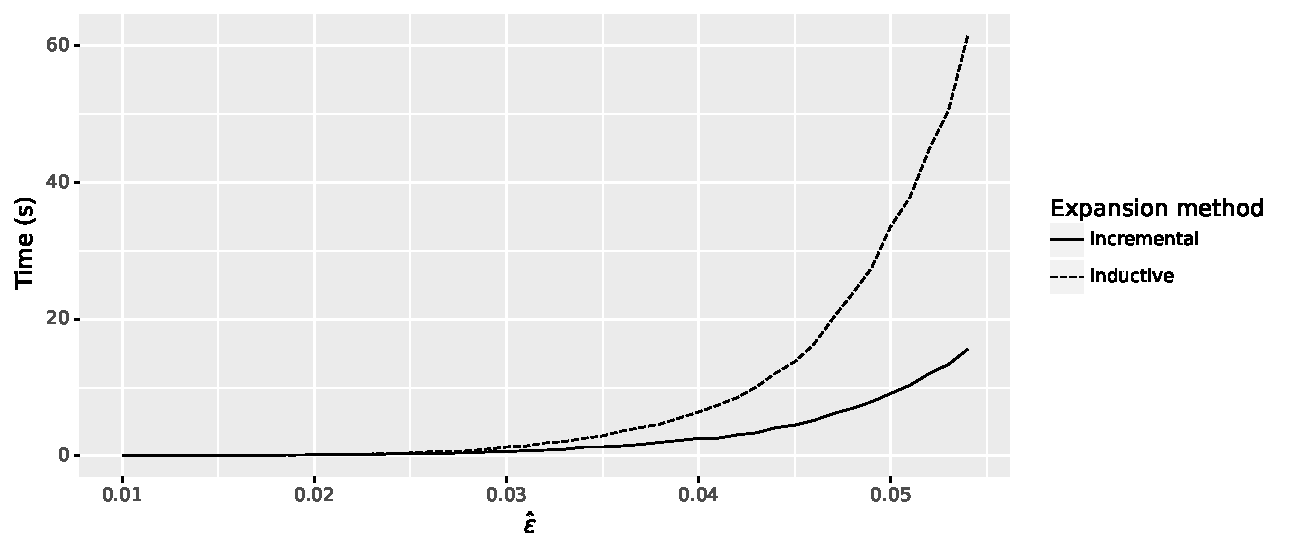
\includegraphics[width=1.2\textwidth]{content/4-comp-top/images/1-expansion-methods}
    }
    \caption{A plot of the performance of two expansion methods (with varying $\varepsilon$): the inductive algorithm and the incremental algorithm. The test set is is the noisy unit circle (with radius fluctuation 0.1) and the expansion is calculated up to 10 dimensions.}
    \label{fig:expansion-methods}
\end{figure}

Figure \ref{fig:expansion-methods} shows the results of experiment (iii) and shows that the incremental algorithm outperforms the inductive algorithm significantly, even though we saw the inductive algorithm perform slightly better for lower values of $\hat\varepsilon$.

To conclude, the incremental algorithm is the best investigated algorithm for expansion, and the sklearn methods outperform the brute-force solution. We again highlight the need for further research investigating hierarchical navigable small-world networks in this context. 

% \begin{definition}[Clustering coefficient]
%     Let $G$ be an undirected graph. The \emph{local clustering coefficient} of a vertex $v \in V(G)$ is given as
%     \[ C_G(v) = \frac{2 \lvert E(N_G(v)] \rvert}{\deg{v} (\deg{v} - 1)}. \]
%     The \emph{network average clustering coefficient} of $G$ is the average local clustering coefficients over all of the vertices in $G$:
%     \[ \overline C_G = \frac1{\lvert V(G) \rvert} \sum_{v \in V} C_G(v). \]
% \end{definition}

% We introduce the graph property of \emph{small-worldness}: a graph $G = (V,E)$ may be described as a \emph{small-world graph} if for each $u, v \in V$, $\E[d(u,v)] \propto \log^k{\lvert V \rvert}$ for some $k > 1$ and the network average clustering coefficient is not small. This concept is not particularly formal, and we will not formalise it here. However, there have been attempts to measure this property. In particular, \textcite{neal2015making} suggested a measure called the \emph{small-world index}, which we will denote by $\swi_G$. Conceptually, this measure evaluates:
% \begin{enumerate}
%     \item whether the average path length in $G$ is close to that of a random network with the same size and degree distribution (see \cite{erdos1959pmd} for details on this construction); and
%     \item whether the network average clustering coefficient of $G$ is close to that of a lattice network with the same size and degree distribution.
% \end{enumerate}
% It is noted that $\swi_G \in [0,1]$, with $\swi_G$ when $G$ does not have a small-world structure and $\swi_G = 1$ when $G$ has a small-world structure (although this is a theoretical maximum, construction of such a graph has not been seen).

% Let $G = (V,E)$ be an undirected graph and $\gr_G: V^2 \to \N_0$ be such that for $u, v \in V$, $\gr_G(u,v)$ denotes the length of a path from $u$ to $v$ as given by a greedy routing algorithm.
